\chapter{Numerische Untersuchung}
\markboth{5 Numerische Untersuchung}{}
\setcounter{footnote}{4}  %um durchgehende Fußnotennummerierung zu haben, hier die Anzahl der bisherigen Fußnoten eintragen

Für die numerische Untersuchung wurden mehrere Berechnungen der optimalen Politik für bestimmte Kombinationen von Eigenschaften der Produktanfragen und verschiedener Wahrscheinlichkeitsverteilungen durchgeführt. Ziel ist es zu untersuchen, ob durch die Möglichkeit der Lagerhaltung eine Veränderung in der optimalen Politik resultiert und sofern es eine Veränderung gibt, in welcher Ausgestaltungsform diese eintritt. Die Ergebnisse der Berechnungen, die in dieser Arbeit vorgestellt sind, wurden mithilfe des Clustersystems an der Leibniz Universität Hannover berechnet. Tabelle \ref{Hardware} zeigt die verwendete Rechnersysteme, wobei eine Berechnung jeweils auf einem Knoten der verfügbaren Rechnersysteme durchgeführt wurde.

\begin{table}[h!]
\renewcommand{\arraystretch}{1.5}
  \begin{center}
  \begin{small}
    \caption{Überblick über Publikationen des traditionellen Konzepts des Revenue Managements in der Fertigungsindustrie}  \label{Hardware}
    \vspace*{3mm}
    \begin{tabular}{llp{6cm}p{1.5cm}p{1.5cm}}   %hier die Spaltenausrichtung, -breite, -begrenzung und -anzahl eintragen
     Cluster & Knoten  & Prozessoren & Kerne/ Knoten  & Speicher/ Knoten (GB) \\  \hline
  Tane   & 96 & 2x Intel Westmere-EP Xeon X5670 (6-cores, 2.93GHz, 12MB Cache, 95W)  & 12 & 48 \\
   Taurus  & 54 & 2x Intel Westmere-EP Xeon X5650 (6-cores, 2.67GHz, 12MB Cache, 95W)  & 12 &  48 \\
   SMP  & 9 &4x Intel Westmere-EX Xeon E7-4830 (8-cores, 2.13GHz, 24MB Cache, 105W)   & 32 & 256  \\
    & 9 & 4x Intel Backton Xeon E7540 (6-cores, 2.00GHz, 18MB Cache, 105W)   & 24 & 256 \\
      & 3 & 4x Intel Westmere-EX Xeon E7-4830 (8-cores, 2.13GHz, 24MB Cache, 105W)   & 32 & 1024  \\ \hline
    \end{tabular} \\[3mm]
    \end{small}
  %  {\footnotesize \textbf{In Anlehnung an:} \cite{quante2009management}, S. 44.}\\
        % {\footnotesize \textbf{Quelle:} \url{http://www.rrzn.uni-hannover.de/scientific_computing_doku.html} }   %footnotesize liefert Schrift in Größe 10pt
  \end{center}
\end{table}

Die in der Arbeit verwendete Implementierung des Auftragsannahmeproblems im Netzwerk RM mit Lagerhaltungsentscheidung sieht die Berechnung der möglichen Systemzustände und des maximal möglichen Erwartungswerts vor. Mithilfe der möglichen Systemzustände wird die Memofunktion gespeist (Vgl. Kapitel ????), die wiederum bei der Berechnung der Erwartungswerte für die benötigten Systemzustände notwendig ist. Bei der Berechnung der Erwartungswerte handelt es sich um das DP. Zusätzlich erfolgt nach Berechnung der Erwartungswerte die Übertragung und Speicherung der optimalen Politik für jeden Systemzustand in eine Datenbank. Aufgrund der zwei Berechnungsschritte werden für beide Berechnungen jeweils die ermittelten Daten bzw. Berechnungskennzahlen angegeben.  Auf dem Rechnersystem wurden folgende Versionen der verwendeten Software-Pakete genutzt:

\colorbox{hellgrau}{\parbox{14cm}{\texttt{Python Version 2.7.9 (default, Jul  2 2015, 11:24:04) [GCC 4.9.2]\\
Numpy Version 1.9.2\\
Matplotlib Version 1.4.3\\
Pandas Version 0.16.2
}}}

Nachfolgend sind alle berechneten Beispiele anhand von Szenarien dargestellt. Je Szenario gibt es eine Anzahl an Buchungsperioden $T$ und eine Anzahl an Leistungserstellungszeitpunkten $\hat T$. In dieser Arbeit wird nur eine Ressource $h\in\mathcal{H}$ betrachtet, was sich ebenfalls in den Szenarien widerspiegelt. Für einen jeden Leistungserstellungszeitpunkt $\hat t \in \hat T$ gibt es eine Anzahl an Kapazitäten $c_h^{\hat t}$, einen Lagerbestand $y_h^{\hat t}$ und einen maximal möglichen Lagerbestand $y_h^{{\hat t},max}$ der Ressource $h=1$. Die unterschiedlichen Produktanfragen $j\in\mathcal{J}$ haben dabei einen individuellen Ertrag $r_j$, einen Parameter für die Inanspruchnahme bzw. Bestandsveränderung der Kapazitäten $a_hj$ der Ressource $h=1$ und einen Zeitpunkt der Leistungserstellung $\hat t$. Die Szenarien besitzen für die Buchungsperioden $t\in T$ eine bestimmte Wahrscheinlichkeitsverteilung $p_j(t)$ über den Auftragseingang einer jeden Produktanfrage $j\in\mathcal{J}$. Die Verteilungen ist jeweils beim Produkt $j$ angegeben und über alle Produkte $j\in\mathcal{J}$ des jeweiligen Szenarios als grafischer Kurvenverlauf abgebildet.

\begin{table}[h!]
\renewcommand{\arraystretch}{1.5}
  \begin{center}
    \caption{Szenario 1}  \label{S1}
    \vspace*{3mm}
    \begin{tabular}{l l l l l l}   %hier die Spaltenausrichtung, -breite, -begrenzung und -anzahl eintragen
    $T$ & $\hat T$  & $h$ & $c_h^{\hat t}\forall \hat{t}\in{\hat T}$ & $y_h^{\hat t}\forall \hat{t}\in{\hat T}$  & $y_h^{{\hat t},max}\forall \hat{t}\in{\hat T}$  \\  \hline
100 & 5 & 1 & 1 & 0 & 2  \\ \hline
    \end{tabular} \\[3mm]
        \begin{tabular}{p{1cm} p{1cm} p{1cm}  p{1cm} p{6cm}}   %hier die Spaltenausrichtung, -breite, -begrenzung und -anzahl eintragen
    $j$ & $r_j$  & $a_{1j}$ & $\hat t$ & Verteilung $p_j(t)$ \\  \hline
1 & 100 & 1 & 1 & Linear verlaufend (0.09)   \\
2 & 1000 & 1 & 1 & Linear verlaufend (0.09)  \\
3 & 100 & 1 & 2 & Linear verlaufend (0.09)  \\
4 & 1000 & 1 & 2 & Linear verlaufend (0.09)  \\
5 & 100 & 1 & 3 & Linear verlaufend (0.09)  \\
6 & 1000 & 1 & 3 & Linear verlaufend (0.09)  \\
7 & 100 & 1 & 4 & Linear verlaufend (0.09)  \\
8 & 1000 & 1 & 4 & Linear verlaufend (0.09)  \\
9 & 100 & 1 & 5 & Linear verlaufend (0.09)  \\
10 & 1000 & 1 & 5 & Linear verlaufend (0.09)  \\ \hline
    \end{tabular} \\[3mm]
     \begin{tabular}{p{7cm}p{5cm}} \hline
     Rechenzeit Systemzustände (h): & \texttt{0:00:00.170329} \\
     Anzahl möglicher Systemzustände: & \texttt{785376} \\
     Anzahl benötigter Systemzustände: & \texttt{76397} \\ 
     Rechenzeit DP (h): & \texttt{16:24:47.128239} \\ 
          Max. Erwartungswert (GE): & \texttt{10858.2} \\ \hline
         \end{tabular} \\[3mm]
  %  {\footnotesize \textbf{In Anlehnung an:} \cite{quante2009management}, S. 44.}\\
        % {\footnotesize \textbf{Quelle:} \url{http://www.rrzn.uni-hannover.de/scientific_computing_doku.html} }   %footnotesize liefert Schrift in Größe 10pt
  \end{center}
\end{table}

Im ersten Szenario werden über einen Buchungszeitraum $T=100$ insgesamt zehn Produktanfragen $j\in\mathcal{J}$ betrachtet. Jeweils zwei Produktanfragen $j$ sind für eine der fünf möglichen Leistungserstellungen vorgesehen und die Anfragen wechseln sich dabei jeweils zwischen dem möglichen Ertrag $r_j=100$ und $r_j=1000$ ab. Die Wahrscheinlichkeitsverteilung einer jeden Produktanfrage verläuft dabei linear mit dem konstanten Wert $p_j(t)$ über den Buchungshorizont $T$, wobei mit Überschreitung der zur Produktanfrage $j$ zugehörigen Leistungserstellung $\hat t$ die Eintrittswahrscheinlichkeit der Produktanfrage auf $p_j(t)=0$ sinkt (Vgl. Abbildung \ref{SB1}).

\begin{figure}[h!]
  \begin{center}
    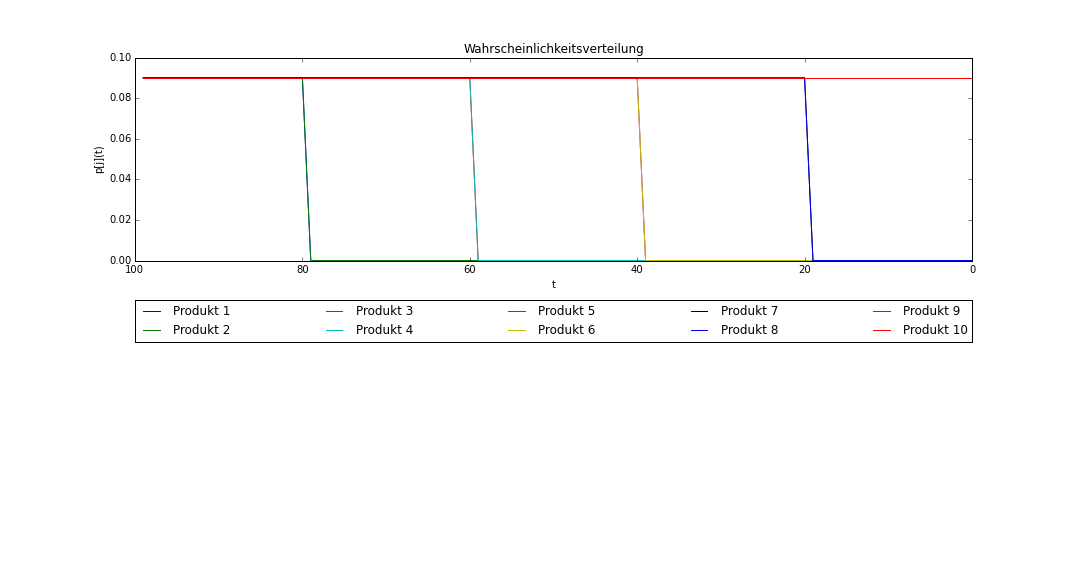
\includegraphics[width=80mm, trim=300pt 180pt 300pt 50pt]{SBilder/1.png}
    \caption{Wahrscheinlichkeitsverteilung Szenario 1}  \label{SB1}
       % {\footnotesize \textbf{Quelle:} ????} 
    %{\footnotesize \textbf{Legende:} Annahme einer Produktauftrag entspricht '$j$', KA='Kein Auftrag'} 
  \end{center}
\end{figure}

\begin{table}[h!]
\renewcommand{\arraystretch}{1.5}
  \begin{center}
    \caption{Auswertung des Szenarios 1}  \label{AS1}
    \vspace*{3mm}
    %%%%%%%%%%%%%%% d[0]
    \begin{tabular}{l l l l l l l l l l l l }  \hline 
         $j$ & 0 & 1  & 2 & 3 & 4  & 5 & 6 & 7 & 8 & 9 & 10  \\  
$d_{0}$ &  57767 &  1461 &  0 &  5048 &  0 &  7960 &  0 &  3367 &  0 &  0 &  0 \\
\hline
    \end{tabular} \\[3mm]
        \begin{tabular}{ l p{2.5cm} p{2.5cm} p{2.5cm} p{2.5cm} }   \hline    %%%%%%%%%%%%%%% d[0]
    $d_j$ & Auftrags\-ablehnung (0) & Auftrags\-annahme (1)  & Lager\-entnahme (2) & Lager\-produktion (3)\\\hline 
$d_{1}$  &  74038 &    104 &    0 &  1461 \\
$d_{2}$  &  73850 &    292 &    0 &  1461 \\
$d_{3}$  &  69657 &    208 &    528 &  5210 \\
$d_{4}$  &  60889 &    404 &  11262 &  3048 \\
$d_{5}$  &  65333 &    304 &   1136 &  8830 \\
$d_{6}$  &  46350 &    659 &  24820 &  3774 \\
$d_{7}$  &  69725 &    216 &   2583 &  3079 \\
$d_{8}$  &  27421 &  10707 &  37475 &   0 \\
$d_{9}$  &  70577 &   2440 &   2586 &   0 \\
$d_{10}$ &  13013 &  29235 &  33355 &   0 \\
          \hline
   \end{tabular} \\[3mm]
     \end{center}
\end{table}

Tabelle \ref{S1} zeigt die verwendeten Parameter des Szenarios und das Ergebnis der Berechnung. Das vollständige Ergebnis ist im Anhang ??? nachzulesen. Tabelle \ref{AS1} zeigt die Auswertung der optimalen Politik die sich aufgrund der Parameter und der Wahrscheinlichkeitsverteilung des Szenarios 1 ergeben. Es handelt sich um eine Auswertung der absoluten Anzahl der Entscheidungen für die optimale Politik sofern keine Anfrage eintrifft ($d_0$) und sofern Anfragen eintreffen ($d_j\forall j \in\mathcal{J}$). Wie in der Tabelle \ref{AS1} zu erkennen, werden nur die Bestandsveränderungsparameter $a_j$ mit niedrigem Ertrag $r_j$ für eine mögliche Lagerhaltungsentscheidung verwendet. Dabei kann die Annahme getroffen werden, dass bei fortschreiten des Buchungshorizonts $T$ die Entscheidung über eine mögliche Lagerproduktion öfters getroffen wird. Bei der optimalen Politik $d_j$ ergibt sich ein ähnliches Bild. Tendenziell werden öfters Anfragen mit niedrigem Ertrag abgelehnt und eine Lagerproduktion durchgeführt. ....

















